\chap{Discussion}
Is possible to say that the obtaiend results are achieving most of the initil goals of this project. 
Like reported in the introduction part [\ref{Introduction}], the two main goals of this work were:\vspace{-2mm}
\begin{itemize}
 \item Implement a web application that provides a scheduler.
 \item Apply the development agile process.
\end{itemize}

The resulting web application actually provides an online scheduler that contains several utilities and functions. Almost all the user stories that were supposed to be realized have been correctly implemented. In particular, the implemented models [\ref{Models}] and the relations between them allowed to reach the main objectives reported during the Introduction part [\ref{Introduction}], like for example let a person be able to create a calendar, fill it with events, share it with an another person and even decide to be updated about changes in an another user's schedule.

Further more, during the whole development process the agile approach had a high consideration and priorization from all the members of the team. Has been actually possible to see a big improvement about the agile process application between the beginning and the end of this work.

In the next section is possible to check out the evaluations about the obtained results and the main limitations found during the project development.
\newpage

\section{Evaluation and Limitations}
\vspace{-5mm}
\label{Evaluation}
The following list reports the main limitations that have been encountered during the implementation process.
\vspace{-5mm}
\begin{itemize}
\item Time limitation has probably been the biggest issue. Working on a project with several people means that you have to somehow find a way to combine different schedules, that is not always that easy. Also a quite short project deadline implies a limitated extra features implementation.
\item Limited amount of previous knowledges and experience about both Ruby on Rails and agile process imply that each single member of the team, mainly during the first part of the work, had to document himself about it. It means a significant investment of time and effort focused about get knowledge and less about web application's extra features. 
\end{itemize}

Despite of the limitations that have been reported above here, every single member of this team learnt many lessons from this work. \\
Below here are reported the most significant:
\vspace{-5mm}
\begin{itemize}
\item Several new knowledges and experience about agile development process, in particular how to handle group project issues such as communication between the members and tasks assignment. 
\item Improved abilities about Git usage, since it has been an indispensable instrument during the whole work.
\item First but really complete approach with framework Ruby on Rails, that also provided a wide overview about web application development.
\end{itemize}

\newpage

\section{Team efforts}
\vspace{-5mm}
One of the most important thing during the whole development process was an efficient assignment of the tasks between the team members and at the same time let everyone put the same effort into the project.
How it's possible to see in the following graphic, there has been a quite constant effort and work on the project.

\begin{figure}[H]
	\centering
    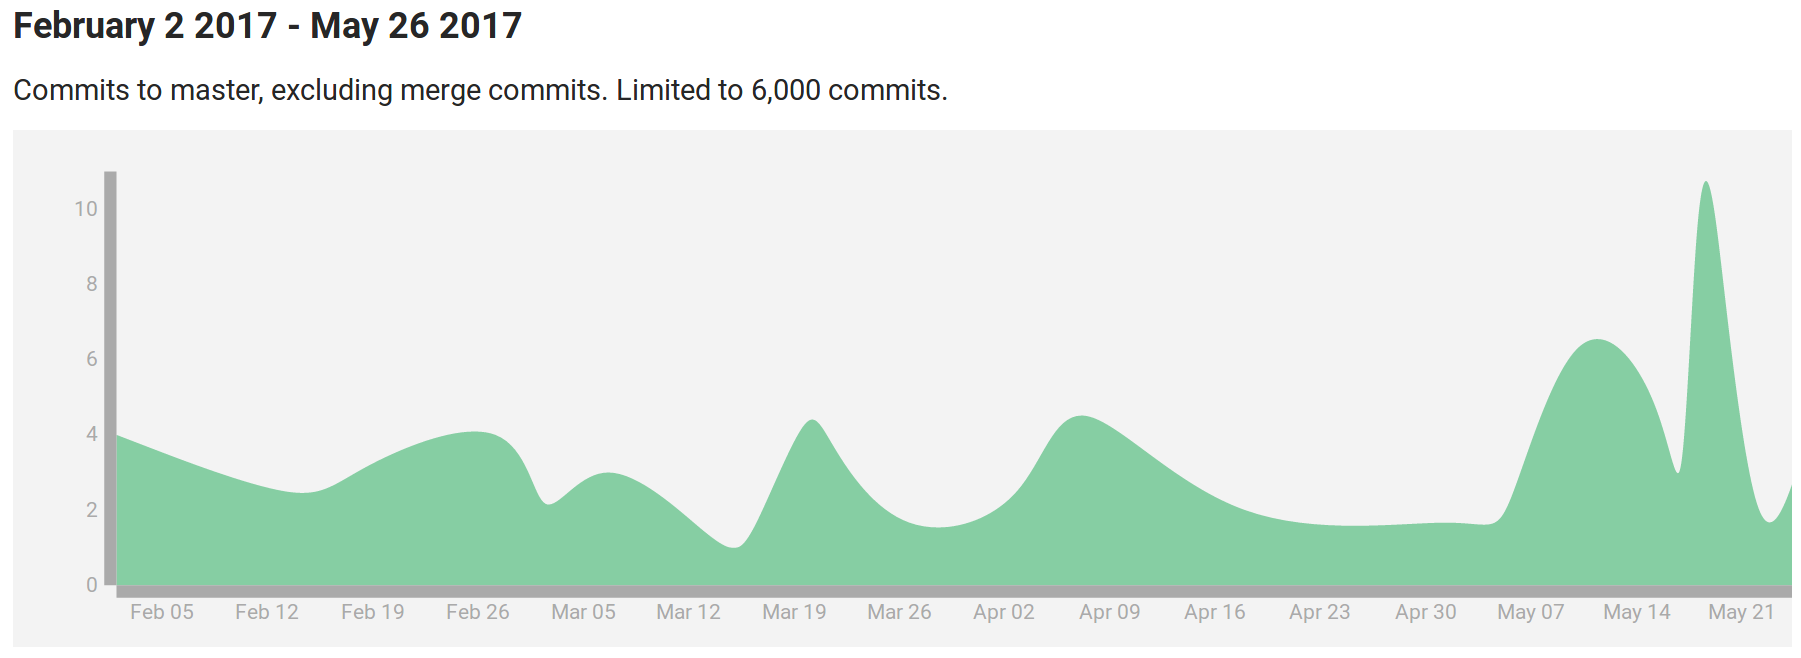
\includegraphics[trim={0 0 0 0},clip,width=1\textwidth]{Files/commitsToMaster.png}
    \caption{Commits to master, excluding merge commits.\\ \textbf{Source:} https://inf2900v17.cs.uit.no/team1/coffee-overflow/graphs/master}
    \label{fig: MVC}
\end{figure}

A good teamwork and effort provided a significant help to the development process. Below here are reported some actual examples of collaboration between team members:
\begin{itemize}

\item If a team mate was not able to attend a group meeting, the other members were sending him a summarize containing the main topics and conclusion of the meeting.
\item If a team mate had a problem related with the project, the other members were always available to help him via chat or even to meet in order to solve it.
\item Quick responses within the group chat by all the team members.
\end{itemize}





